编写一个源码树内LLVM IR回归测试非常简单,用测试指令注释IR文件:

\begin{tcolorbox}[colback=white,colframe=black]
\tt
\zihao{-5}
; RUN: opt < \%s -instcombine -S -o - | FileCheck \%s \\
target triple = "x86\_64-unknown-linux" \\
define i32 @foo(i32 \%c) \{ \\
\hspace*{0.3cm}entry: \\
\hspace*{0.3cm}; CHECK: [[RET:\%.+]] = add nsw i32 \%c, 3 \\
\hspace*{0.3cm}; CHECK: ret i32 [[RET]] \\
\hspace*{0.3cm}\%add1 = add nsw i32 \%c, 1 \\
\hspace*{0.3cm}\%add2 = add nsw i32 \%add1, 2 \\
\hspace*{0.3cm}ret i32 \%add2 \\
\}
\end{tcolorbox}

这个脚本检查InstCombine(由前面代码中显示的\texttt{-instcombine}命令行选项触发)是否将两个后续的算术相加简化为一个指令。将该文件放入llvm/test下的任意文件夹后,当执行llvm-lit工具时,脚本将会自动选中,并作为回归测试的一部分运行。

尽管很方便,但几乎不能帮助您在树外项目中使用LIT。当其他项目需要一些端到端测试工具(比如:格式转换器、文本处理器、检测程序,还有编译器)时,树外LIT尤其好用。本节将向您展示如何将LIT引入到树外项目中,然后提供LIT运行流程的完整描述。

\subsubsubsection{3.2.1\hspace{0.2cm}准备示例项目}

本节中,将使用源码树外的CMake项目。这个示例项目构建了一个工具\texttt{js-minifier},它用于简化JavaScript代码。我们将转换以下JavaScript代码:

\begin{lstlisting}[style=styleJavaScript]
const foo = (a, b) => {
	let c = a + b;
	console.log(`This is ${c}`);
}
\end{lstlisting}

可以将其转换成一些语义等价的代码,并尽可能短:

\begin{lstlisting}[style=styleJavaScript]
const foo = (a,b) => {let c = a + b; console.log(`This is ${c}`);}
\end{lstlisting}

本节的目标不是了解如何编写这个\texttt{js-minifier},而是如何创建一个LIT测试环境,从而对这个工具进行测试。

示例项目的文件夹结构如下所示:

\begin{tcolorbox}[colback=white,colframe=black]
\tt
\zihao{-5}
/JSMinifier \\
\hspace*{0.3cm}|\_\_\_ CMakeLists.txt \\
\hspace*{0.3cm}|\_\_\_ /src \\
\hspace*{0.3cm}|\hspace{1cm}|\_\_\_ js-minifier.cpp \\
\hspace*{0.3cm}|\hspace{1cm}|\_\_\_ /test \\
\hspace*{0.3cm}|\hspace{2.3cm}|\_\_\_ test.js \\
\hspace*{0.3cm}|\hspace{2.3cm}|\_\_\_ CMakeLists.txt \\
\hspace*{0.3cm}|\_\_\_ /build
\end{tcolorbox}

src文件夹下的文件包含js-minifier的源代码(这里不打算介绍)。这里我们关注的是用于测试js-minifier的文件,位于/test文件夹下(目前只有一个文件test.js)。

本节中,我们将建立一个测试环境,当我们在CMake /build文件夹下运行llvmlit(测试驱动程序和本节的主要字符)时,就会打印测试结果,像这样:

\begin{tcblisting}{commandshell={}}
$ cd build
$ llvm-lit -sv .
-- Testing: 1 tests, 1 workers –
PASS: JSMinifier Test :: test.js (1 of 1)
Testing Time: 0.03s
  Expected Passes : 1
\end{tcblisting}

这显示了多少测试用例通过了测试,以及具体是哪些测试用例。

下面是测试脚本test.js:

\begin{lstlisting}[style=styleJavaScript]
// RUN: %jsm %s -o - | FileCheck

// CHECK: const foo = (a,b) =>
// CHECK-SAME: {let c = a + b; console.log(`This is ${c}`);}
const foo = (a, b) => {
	let c = a + b;
	console.log(`This is ${c}`);
}
\end{lstlisting}

可以看到,这是一个简单的测试过程,运行js-minifier工具——由\texttt{\%jsm}指令将被js-minifier可执行文件的实际路径所替代——并使用CHECK和CHECK-SAME的指令,用FileCheck检查运行结果。

这样,我们的示例项目就完成了。在结束准备工作之前,我们还需要创建最后一个工具。

因为试图减少对LLVM源代码树的依赖,所以要使用PyPi存储库中可用的LIT包(即pip命令行工具)重新创建\texttt{llvm-lit}工具。你所需要做的就是安装这个包:

\begin{tcblisting}{commandshell={}}
$ pip install --user lit
\end{tcblisting}

最后,用下面的脚本包装这个包:

\begin{lstlisting}[style=stylePython]
#!/usr/bin/env python
from lit.main import main
if __name__ == '__main__':
	main()
\end{lstlisting}

现在,我们无需构建LLVM树,就可以使用LIT了。接下来,我们将创建一些LIT配置脚本,这些脚本将驱动整个测试流。

\subsubsubsection{3.2.2\hspace{0.2cm}对LIT进行配置}

本小节中,将展示如何编写LIT配置脚本。这些脚本描述了测试过程——测试文件在哪里、如何配置测试环境(例如,需要导入某些工具)、出现故障时的应对策略等。学习这些技能可以极大地改善在LLVM之外的地方使用LIT的体验。这就开始吧!

\begin{enumerate}
\item 在/JSMinifier/test文件夹中,创建一个名为lit.cfg.py的文件:

\begin{lstlisting}[style=stylePython]
import lit.formats

config.name = 'JSMinifier Test'
config.test_format = lit.formats.ShTest(True)
config.suffixes = ['.js']
\end{lstlisting}

代码为LIT提供了一些信息。这里的配置变量是一个Python对象,当这个脚本加载到LIT的运行时,将使用相应的信息进行替代。使用预定义的字段,本质上就是注册表配置值,可以使用lit.*.py脚本添加相应的定制字段。

config.test\_format字段表示LIT将在shell环境中运行每个测试(以ShTest格式),而config.suffixes字段表示只有文件名后缀为.js的文件才会视为测试用例(就是所有的JavaScript文件)。

\item 写完上一步的代码后,LIT现在需要另外两个信息:测试文件的根路径和工作目录:

\begin{lstlisting}[style=stylePython]
…
config.suffixes = ['.js']
config.test_source_root = os.path.dirname(__file__)
config.test_exec_root = os.path.join(config.my_obj_root,
'test')
\end{lstlisting}

config.test\_source\_root指向/JSMinifier/test。另一方面,config.test\_exec\_root表示工作目录,my\_obj\_root是是一个自定义配置字段的值表示其父文件夹位置,它指向构建文件夹的路径。换句话说,config.test\_exec\_root最终值为/JSMinifier/build/test。

\item 之前在test.js中,使用\texttt{\%jsm}指令作为占位符,其最终会被js-minifier可执行文件的实际/绝对路径所取代。以下几行将设置替换值:

\begin{lstlisting}[style=stylePython]
…
config.test_exec_root = os.path.join(config.my_obj_root, 'test')

config.substitutions.append(('%jsm',
os.path.join(config.my_obj_root, 'js-minifier')))
\end{lstlisting}

这段代码向配置添加了一个config.substitutions字段,它使LIT用/JSMinifier/ build/js-minifier值替换测试文件中出现的每一个\texttt{\%jsm}。这将把所有内容打包到lit.cfg.py中。

\item 现在,创建一个名为lit.site.cfg.py.in的新文件,并将其放在/JSMinifier/test文件夹下。这个文件的第一部分看起来是这样:

\begin{lstlisting}[style=stylePython]
import os
config.my_src_root = r'@CMAKE_SOURCE_DIR@'
config.my_obj_root = r'@CMAKE_BINARY_DIR@'
\end{lstlisting}

神秘的config.my\_obj\_root字段在这里解析,但不指向正常的字符串,它分配到的值为@CMAKE\_BINARY\_DIR@,这个字段将被CMake替换为实际路径,其值与config.my\_src\_root字段一致。

\item 最后,这些信息都放在了lit.site.cfg.py.in里面:

\begin{lstlisting}[style=stylePython]
…
lit_config.load_configure(
	config, os.path.join(config.my_src_root, 'test/
		lit.cfg.py'))
\end{lstlisting}

尽管这段代码非常简单,但还是有点难以理解。简单地说,这个文件最终将具象化到另一个文件中,所有使用两个\texttt{@}包围的变量都将进行解析,并复制到构建文件夹中。在那里,将回调前面步骤中的lit.cfg.py,这将在本节的后面进行解释。

\item 最后,是时候使用CMake的\texttt{configure\_file}函数将那些使用两个\texttt{@}包围的字符串替换为实际值。在/JSMinifier/test/CMakeLists.txt中,在文件中添加以下内容:

\begin{lstlisting}[style=styleCMake]
configure_file(lit.site.cfg.py.in
  lit.site.cfg.py @ONLY)
\end{lstlisting}

\texttt{configure\_file}函数将使用当前CMake中的对应变量的值替换输入文件(lit.site.cfg.py.in)中使用两个\texttt{@}包围的字符串。

例如,假设有一个名为demo.txt.in的文件,其中包含以下内容:

\begin{lstlisting}[style=styleCMake]
name = "@FOO@"
age = @AGE@
\end{lstlisting}

现在,在CMakeLists.txt中使用\texttt{configure\_file}:

\begin{lstlisting}[style=styleCMake]
set(FOO "John Smith")
set(AGE 87)
configure_file(demo.txt.in
			   demo.txt @ONLY)
\end{lstlisting}

前面提到的替换将启动,并生成一个输出文件demo.txt,文件内容如下:

\begin{lstlisting}[style=styleCMake]
name = "John Smith"
age = 87
\end{lstlisting}

\item 回到lit.site.cfg.py.in中,由于\texttt{CMAKE\_SOURCE\_DIR}和\texttt{CMAKE\_BINARY\_DIR}分别指向根源文件夹和构建文件夹。/JSMinifier/build/test/lit.site.cfg.py将包含以下内容:

\begin{lstlisting}[style=stylePython]
import os
config.my_src_root = r'/absolute/path/to/JSMinifier'
config.my_obj_root = r'/absolute/path/to/JSMinifier/build'

lit_config.load_config(
	config, os.path.join(config.my_src_root, 'test/
		lit.cfg.py'))
\end{lstlisting}

\end{enumerate}

至此,我们了解了如何为示例项目编写LIT配置脚本。现在,是时候解释一些关于LIT内部如何工作的细节,以及为什么我们需要这么多文件(lit.cfg.py,lit.site.cfg.py和lit.site.cfg.py)。

\subsubsubsection{3.2.3\hspace{0.2cm}LIT的内部构件}

让我们看看下面的图表,它展示了在我们刚刚创建的演示项目中,运行LIT测试的工作流程:

\hspace*{\fill} \\ %插入空行
\begin{center}
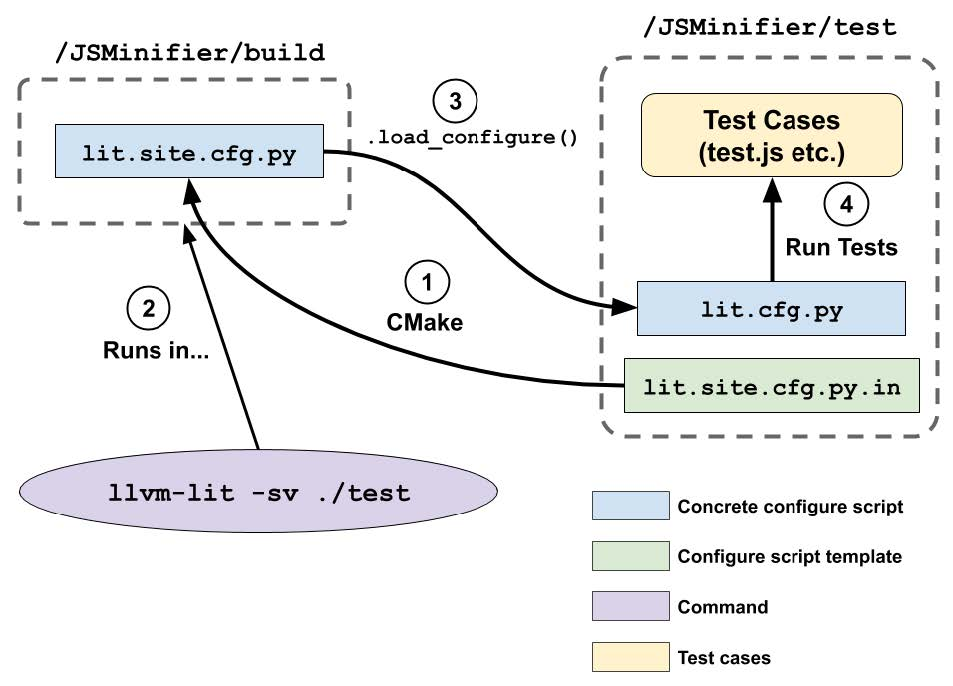
\includegraphics[width=0.9\textwidth]{content/1/chapter3/images/1.jpg}\\
图3.1 -示例项目中LIT的流程
\end{center}

让我们详细地看看这张图:

\begin{enumerate}
\item 将lit.site.cfg.py.in复制至/JSMinifier/build//JSMinifier/build/lit.site.cfg.py,其中包含一些CMake变量值。

\item \texttt{llvm-lit}在/JSMinifier/build中启动,将首先执行lit.site.cfg.py。

\item 然后使用\texttt{load\_configure} Python函数加载主要的LIT配置(lit.cfg.py),并运行所有的测试用例。
\end{enumerate}

这个图中最关键的部分是解释lit.site.cfg.py和lit.site.cfg.py.in的角色:它们有很多参数,比如构建目录的绝对路径,在CMake配置过程完成前都是未知的。因此,将一个弹性脚本(即lit.site.cfg.py)放置在构建目录中,可以将该信息传递给实际的测试运行器。

在本节中,我们了解了如何为自己的树外示例项目编写LIT配置脚本。还了解了LIT在引擎盖下是如何工作的,这可以帮助您在各种各样的项目中使用LIT(除了LLVM)。

下一节中,我们将重点讨论FileCheck,这是一个重要且常用的LIT程序,可以以更高级的模式执行检查。





